\section{Dwi Yulianingsih}
\subsection{Sejarah Phyton}
Phyton adalah sebuah bahasa pemrograman dengan perancangan yang berfokus pada tingkat keterbacaan kode, menggabungkan kapabilitas, kemampuan dan sintaks kode yang sangat jelas. Phyton juga dilengkapi dengan fungsi pustaka atau library standar yang besar dan didukung oleh komunitas yang besar. Phyton dibuat oleh seseorang keturunan belanda yaitu Guido Van Rossum, awalnya pembuatan phyton ini digunakan untuk pembuatan bahasa tingkat tinggi pada sebuah sistem operasi. Phyton telah digunakan oleh perusahaan-perusahaan untuk membuat perangkat lunak komersil. Pemrograman bahasa python merupakan pemrogram gratis atau freeware, sehingga bisa dikembangkan, dan tidak memiliki batasan dalam peng-copy-an dan didistribusikan. Terdapat beberapa layanan yang diberikan dalam phyton lengkap dengan source kodenya, debugger dan profiler, antarmuka, fungsi sistem, GUI, dan database-nya. Python dapat digunakan untuk berbagai Sistem Operasi, yang diantaranya Unix (linux), PCs (DOS, Windows, OS/2), Machintosh dan sebagainya.


\subsection{Instalasi Anaconda}
\begin{enumerate}
    \item Kita harus menyiapkan instalasi anaconda, kita dapat mendownload nya melalui internet.
    \item Kemudian kita bisa mengklik installer yang telah kita miliki dan tunggu.
    \begin{figure}[!htbp]
        \centering
        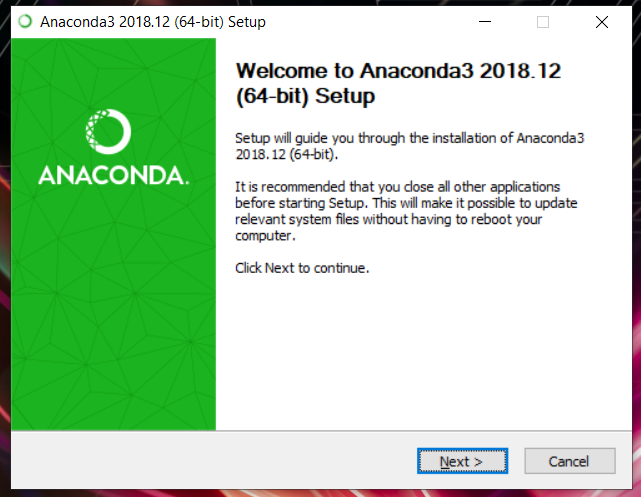
\includegraphics[width=3cm,height=3cm]{figures/1.png}
        \caption{gambar1}
        \label{awal}
        \end{figure}

    \item Lalu pada tampilan seperti gambar di bawah klik next.
    \begin{figure}[!htbp]
        \centering
        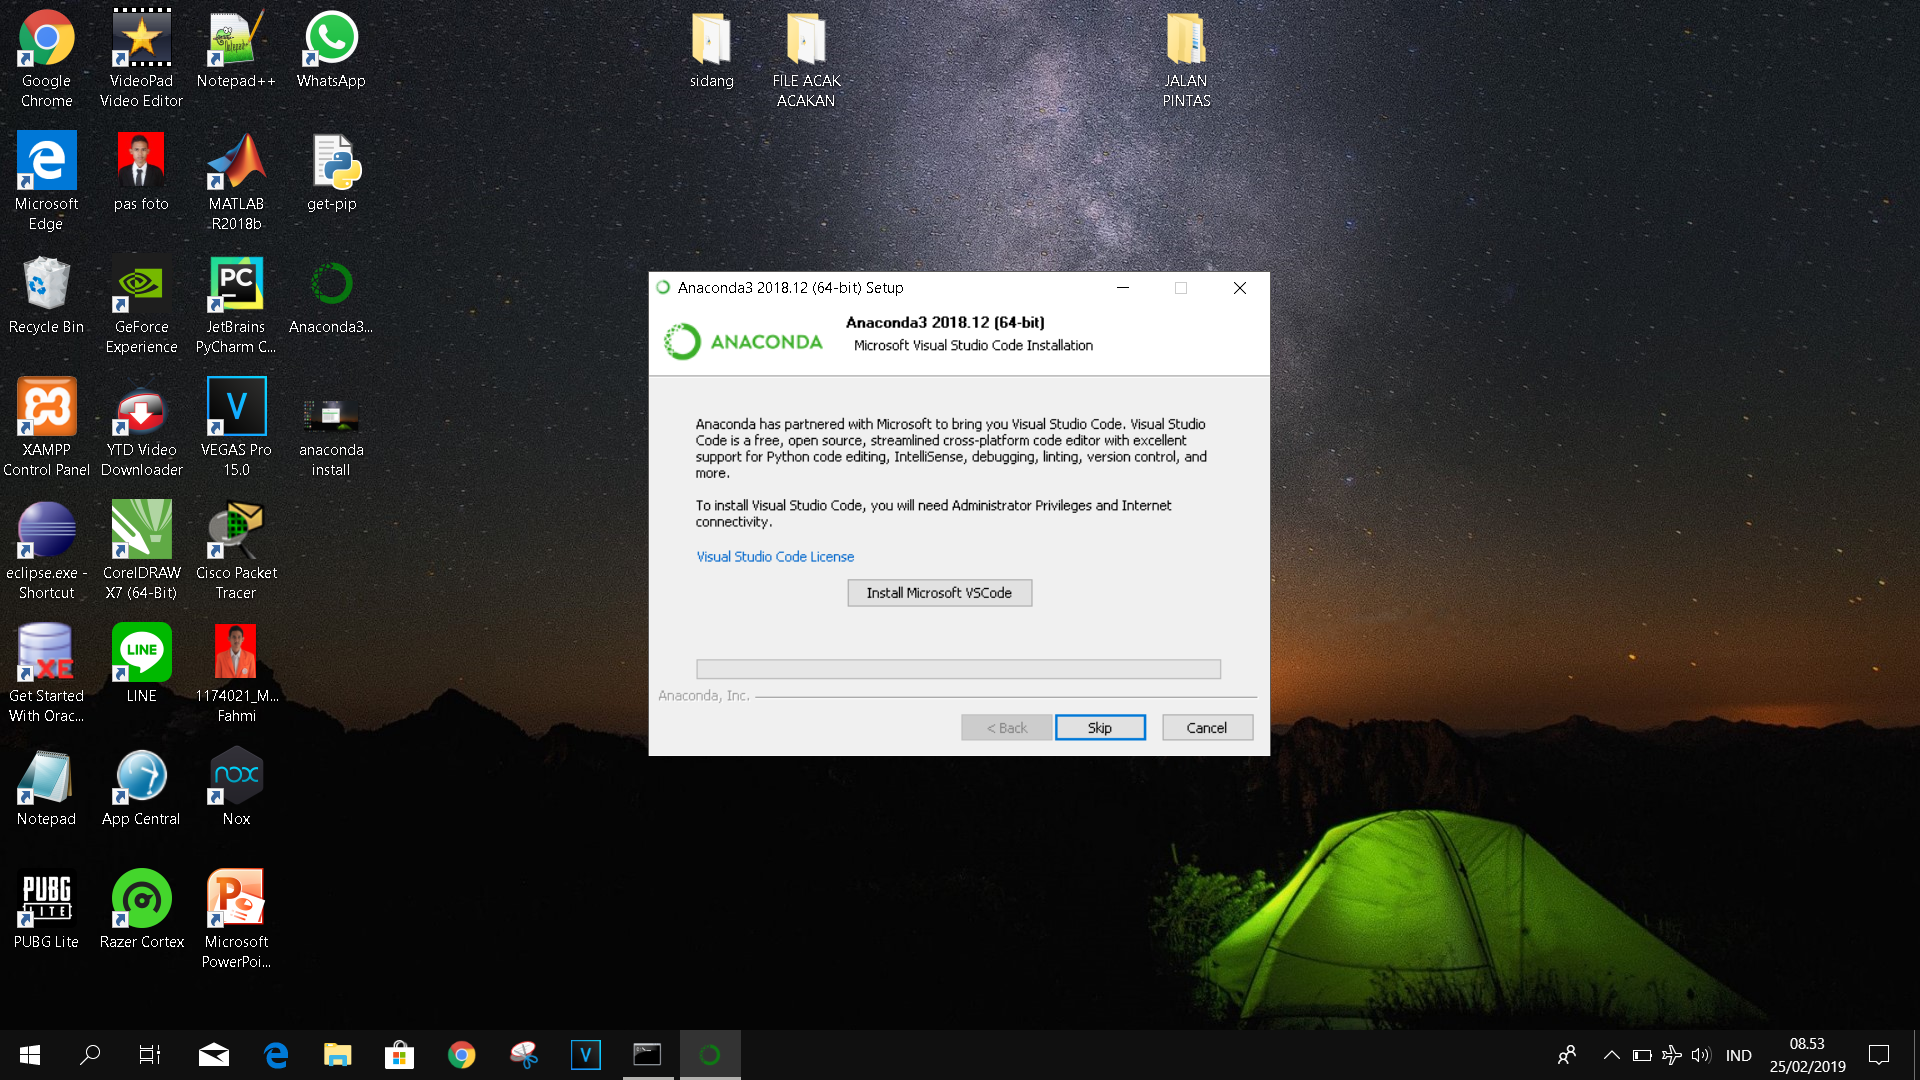
\includegraphics[width=3cm,height=3cm]{figures/2.png}
        \caption{gambar2}
        \label{next}
        \end{figure}

    \item Setelah itu setujui lisensi yang ada dengan mengklik I Agree
    \begin{figure}[!htbp]
        \centering
        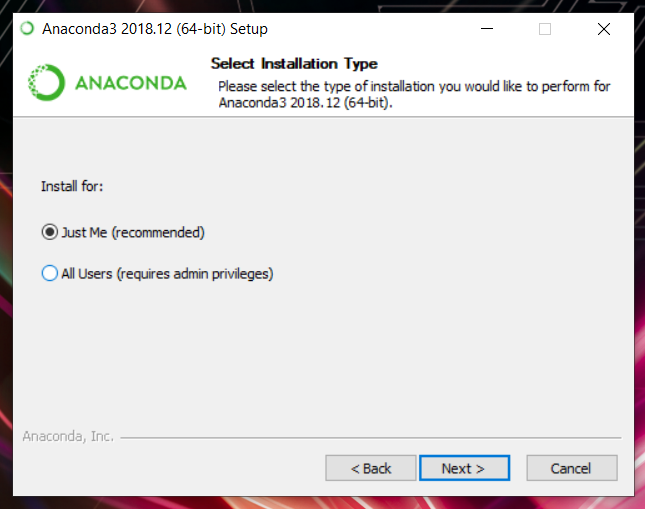
\includegraphics[width=3cm,height=3cm]{figures/3.png}
        \caption{gambar3}
        \label{lisensi}
        \end{figure}

    \item Tunggu instalasi selesai, lalu klik skip
    \begin{figure}[!htbp]
        \centering
        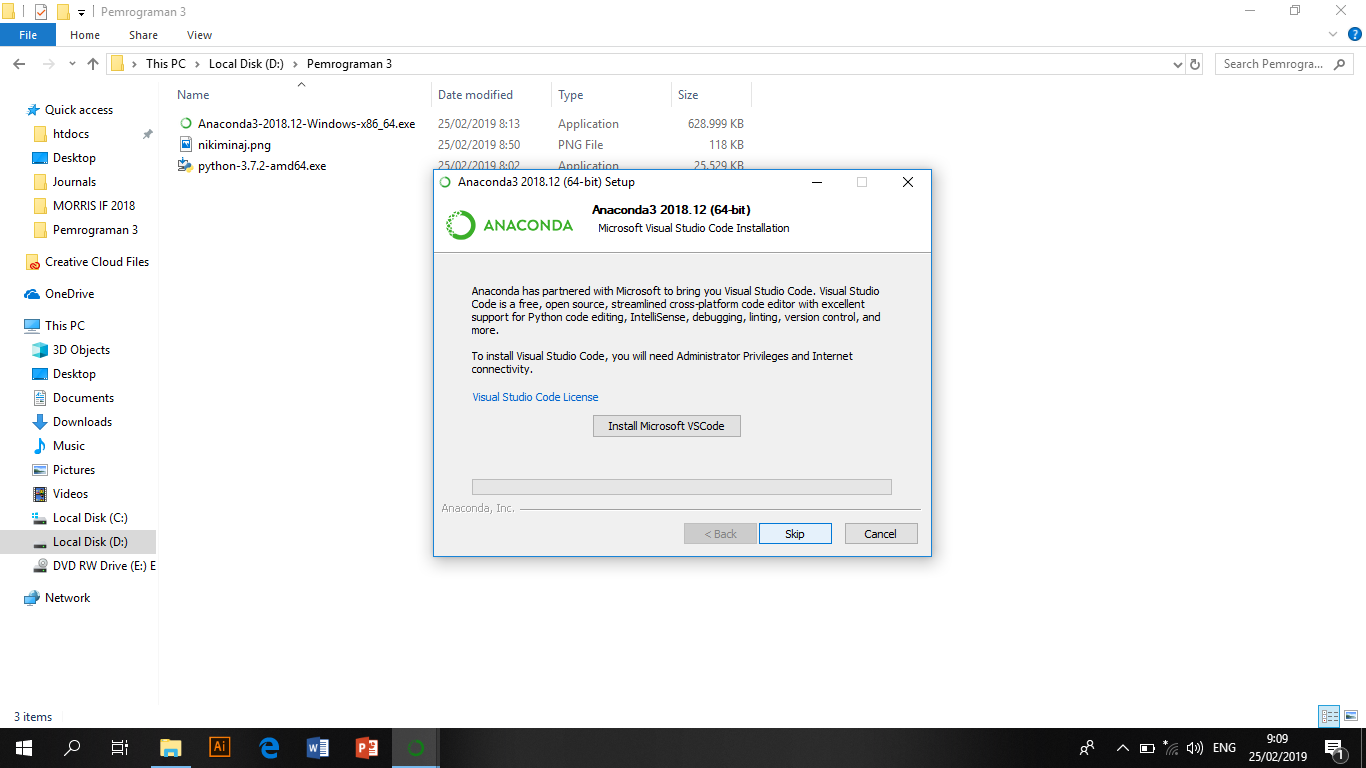
\includegraphics[width=3cm,height=3cm]{figures/4.png}
        \caption{gambar4}
        \label{skip}
        \end{figure}

    \item setelah itu klik finish, dan selesai yeay
    \begin{figure}[!htbp]
        \centering
        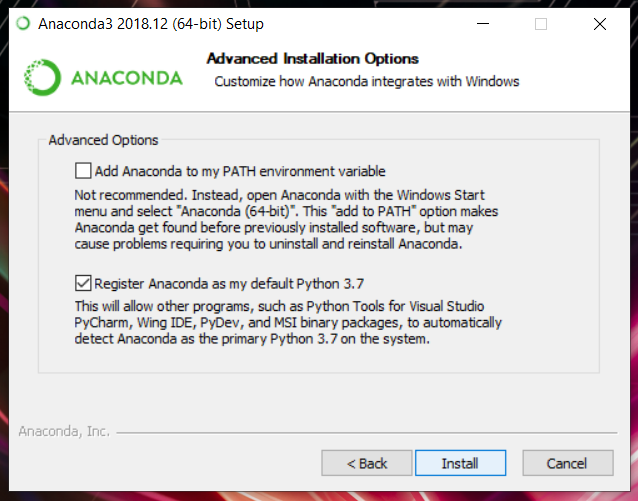
\includegraphics[width=3cm,height=3cm]{figures/5.png}
        \caption{gambar5}
        \label{selesai}
        \end{figure}
\end{enumerate}

\subsection{Menggunakan Spyder}
berikut adalah contoh dalam menggunakan spyder
\begin{figure}[!htbp]
    \centering
    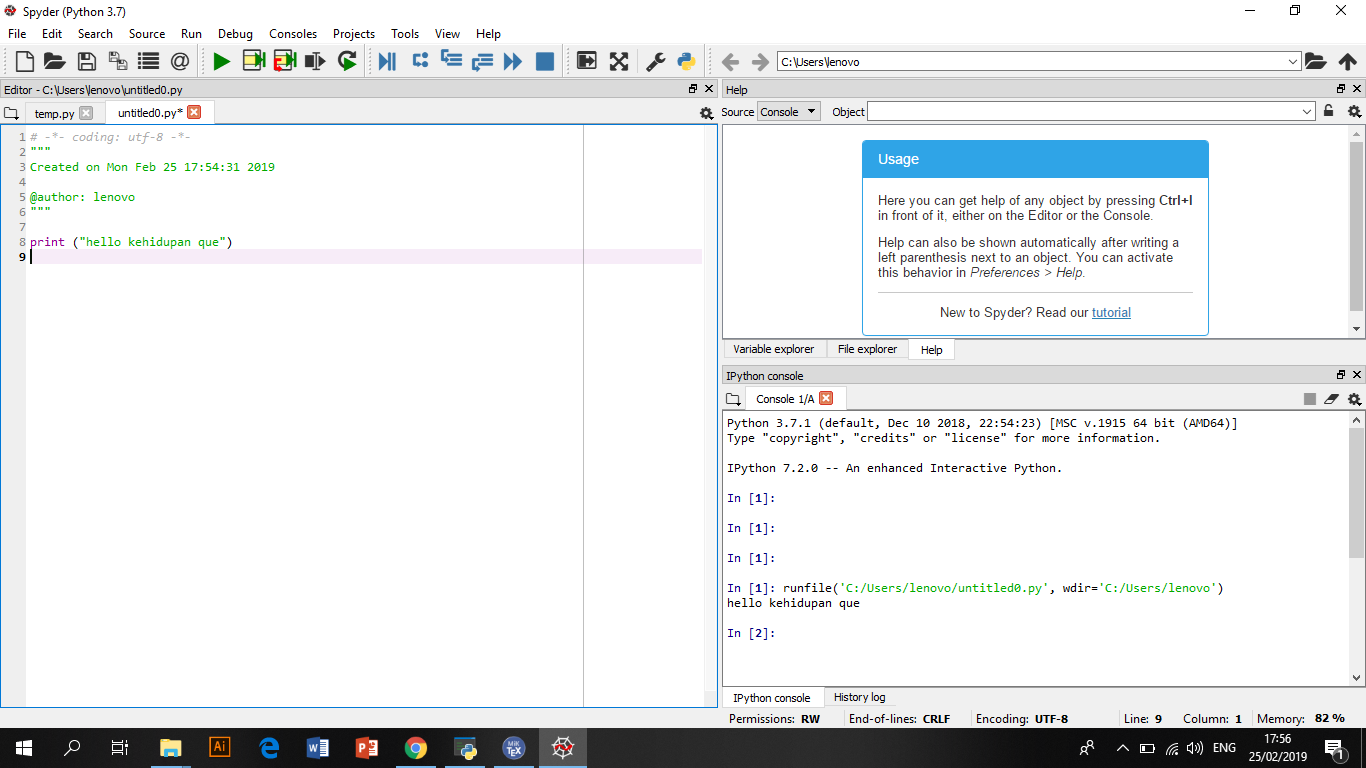
\includegraphics[width=3cm,height=3cm]{figures/6.png}
    \caption{gambar6}
    \label{spyder}
    \end{figure}
	
\Section{Dwi Septiani Tsaniyah}
\subsection{sejarah}
\section{Sejarah Python}

Python dikembangkan oleh Guido van Rossum sebagai bahasa pemrograman ABC pada tahun 1990 di Stichting Mathematisch Centrum (CWI) di Amsterdam. Versi terbaru yang dirilis oleh CWI adalah 1.2.

Pada 1995, Guido pindah ke CNRI di Virginia, AS, dan terus mengembangkan Python. Versi terakhir yang dirilis 1.6. Pada tahun 2000, insinyur Guido dan Python menjadi perusahaan komersial untuk BeOpen.com dan menciptakan BeOpen PythonLabs. Python 2.0 dirilis oleh BeOpen. Setelah menghapus Python 2.0, beberapa anggota Guido dan PythonLabs pindah ke DigitalCreations.

Saat ini, pengembangan Python sedang dilanjutkan oleh sekelompok programmer yang dikoordinir oleh Guido dan Yayasan Perangkat Lunak Python. Python Software Foundation, versi 2.1, memiliki hak cipta Python, dan Python adalah organisasi nirlaba yang memblokir kepemilikan perusahaan komersial. Saat ini, distribusi Python telah mencapai versi 2.7.14 dan versi 3.6.3

Program televisi Guido Monty Python Flying Circus telah dinamai nama Python oleh Guido sebagai bahasa ciptaannya. Oleh karena itu, sering kali ungkapan khas suatu acara sering muncul dalam korespondensi antara pengguna Python.

\section{sejarah}
Python diciptakan oleh Guido van Rossum pertama kali di Scitchting Mathematisch Centrum (CWI) di Belanda pada awal tahun 1990-an. Bahasa python terinspirasi dari bahasa pemrograman ABC. Sampai sekarang, Guido masih menjadi penulis utama untuk python, meskipun bersifat open source sehingga ribuan orang juga berkontribusi dalam mengembangkannya.

Pada 1995, Guido pindah ke CNRI di Virginia Amerika sambil terus mengembangkan Python. Versi terakhir yang dirilis adalah 1.6. Pada tahun 2000, pengembang inti Guido dan Python pindah ke BeOpen.com yang merupakan perusahaan komersial dan membentuk BeOpen PythonLabs. Python 2.0 dirilis oleh BeOpen. Setelah menghapus Python 2.0, Guido dan beberapa anggota tim PythonLabs pindah ke DigitalCreations.

Saat ini pengembangan Python terus dilakukan oleh sekelompok programmer yang dikoordinir oleh Guido dan Python Software Foundation. Python Software Foundation adalah organisasi nirlaba yang dibentuk sebagai pemegang hak cipta intelektual Python sejak versi 2.1 dan dengan demikian mencegah Python dimiliki oleh perusahaan komersial. Saat ini distribusi Python telah mencapai versi 2.7.14 dan versi 3.6.3

Nama Python dipilih oleh Guido sebagai nama bahasa ciptaannya karena kecintaan Guido pada acara televisi Flying Circus Monty Python. Oleh karena itu sering ekspresi khas acara sering muncul dalam korespondensi antara pengguna Python.
\section{Instalasi Anaconda}
\begin{enumerate}
    \item Pastikan Bahwa Python telah terinstal dilaptop anda.
    \item Jika anda belum punya anaconda, kalian bisa download di https://www.anaconda.com/distribution/#download-section
    \item Kemudian buka installer yang telah di download barusan
    \item Klik next
    \begin{figure}[!htbp]
        \centering
        \includegraphics[width=3cm,height=3cm]{figures/Screenshot(219).png}
        \caption{Tampilan Awal}
        \label{awal}
        \end{figure}

    \item Kemudian Klik I Agree
    \begin{figure}[!htbp]
        \centering
        \includegraphics[width=3cm,height=3cm]{figures/Screenshot(221).png}
        \caption{License Agreement}
        \label{License}
        \end{figure}

    \item Kemudian pilih akan di instal untuk siapa, kemudian pilih next
    \begin{figure}[!htbp]
        \centering
        \includegraphics[width=3cm,height=3cm]{figures/Screenshot(222).png}
        \caption{Pemilihan User}
        \label{User}
        \end{figure}

    \item Kemudian tentukan dicretory nya, secara default akan berada di C:\Users\namakomputer\Anaconda3
    \begin{figure}[!htbp]
        \centering
        \includegraphics[width=3cm,height=3cm]{figures/Screenshot(223).png}
        \caption{Pemilihan Direktori Penyimpanan}
        \label{Directory}
        \end{figure}

    \item Kemudian Centang yang register Anaconda as default Python, Kemudian Pilih Next
    \begin{figure}[!htbp]
        \centering
        \includegraphics[width=3cm,height=3cm]{figures/Screenshot(225).jpeg}
        \caption{Pemilihan Opsi}
        \label{opsi}
        \end{figure}

    \item Tunggu Proses Instalasi hingga selesai
    \begin{figure}[!htbp]
        \centering
        \includegraphics[width=3cm,height=3cm]{figures/Screenshot(226).png}
        \caption{Proses Instal}
        \label{Proses}
        \end{figure}

    \item Instalasi telah selesai
    \begin{figure}[!htbp]
        \centering
        \includegraphics[width=3cm,height=3cm]{figures/Screenshot(227).png}
        \caption{Proses Instal Selesai}
        \label{Proses}
        \end{figure}
\subsection
kodingan sederhana Hello Word 

\end{enumerate}
\section{Menggunakan Spyder}
